\documentclass[conference]{IEEEtran}

% --- PACKAGES ---
\usepackage{cite}
\usepackage{amsmath,amssymb,amsfonts}
\usepackage{booktabs} % For high-quality tables
\usepackage{url}      % For URLs in references
\usepackage{graphicx} % For including figures
\usepackage[binary-units=true]{siunitx} % For \SI{}{} commands (e.g., timings)
\usepackage{algorithm} % For algorithm blocks
\usepackage[noend]{algpseudocode} % For algorithm blocks
\usepackage{etoolbox} % For fixing IEEEtran algorithm numbering
% \usepackage{lipsum} % REMOVED dummy text package

% --- Tell LaTeX where to find the images ---
% Assuming images are in the SAME directory as the .tex file.
% \graphicspath{{simulation_results/}} % Use this ONLY if images are in a subfolder

% --- IEEEtran Algorithm Numbering Fix ---
\makeatletter
\let\saved@opargbegintheorem\@opargbegintheorem
\let\@opargbegintheorem\relax
\makeatother
\usepackage{algorithm}
\makeatletter
\let\@opargbegintheorem\saved@opargbegintheorem
\makeatother
% --- End Fix ---


% correct bad hyphenation here
\hyphenation{op-tical net-works semi-conduc-tor}


\begin{document}

% --- TITLE AND AUTHORS ---
\title{An Empirical Study on the Impact of Key Parameters in Federated Learning for Image Classification} % Slightly more specific title

\author{
    \IEEEauthorblockN{Author One Name}
    \IEEEauthorblockA{Department of Computer Science}
    \IEEEauthorblockA{Your University}
    \IEEEauthorblockA{City, Country}
    \IEEEauthorblockA{email@your.university}
    \and
    \IEEEauthorblockN{Author Two Name}
    \IEEEauthorblockA{Department of Computer Science}
    \IEEEauthorblockA{Your University}
    \IEEEauthorblockA{City, Country}
    \IEEEauthorblockA{email@your.university}
    \and
    \IEEEauthorblockN{Author Three Name}
    \IEEEauthorblockA{Department of Computer Science}
    \IEEEauthorblockA{Your University}
    \IEEEauthorblockA{City, Country}
    \IEEEauthorblockA{email@your.university}
}

% make the title area
\maketitle

% --- ABSTRACT ---
\begin{abstract}
Federated Learning (FL) offers a privacy-preserving paradigm for training machine learning models on decentralized data residing on devices like smartphones or sensors. However, the performance of FL systems, particularly the widely used Federated Averaging (FedAvg) algorithm, is known to be sensitive to hyperparameter choices and the inherent statistical heterogeneity (Non-IID nature) of distributed data. This paper presents a detailed empirical investigation, conducted through simulation, into the effects of two critical FedAvg parameters: the client participation fraction (C) and the number of local training epochs (E). Using the MNIST handwritten digit dataset and a standard Convolutional Neural Network (CNN), we systematically evaluate how variations in C and E impact model convergence speed, stability, and final accuracy under both IID and challenging Non-IID data distributions. Our results quantitatively confirm that Non-IID data significantly impedes FedAvg, reducing final accuracy from 99.09\% (IID) to 96.34\% (Non-IID baseline) and introducing substantial training instability. We show that increasing client participation (C=0.5) dramatically improves stability and boosts Non-IID accuracy to 98.43\%, closely approaching IID performance, though at the cost of increased per-round computation. Conversely, we illustrate the complex trade-off associated with local epochs: reducing E (E=1) leads to slow convergence and poor accuracy (93.65\%), while increasing E (E=10) exacerbates client drift and initial instability, despite eventually reaching high accuracy (97.74\%). Furthermore, we demonstrate that a combined strategy of high participation and low local epochs (C=0.5, E=1) provides an effective balance, achieving robust convergence, high accuracy (97.42\%), and reasonable efficiency. These findings offer practical insights into parameter tuning for mitigating Non-IID challenges in FL systems.
\end{abstract}

% no keywords
\IEEEpeerreviewmaketitle


% --- INTRODUCTION ---
\section{Introduction}
The proliferation of mobile devices, IoT sensors, and edge computing has led to an unprecedented explosion of data generated outside traditional data centers \cite{b21}. This distributed data represents a rich resource for training sophisticated machine learning models, enabling applications ranging from personalized recommendations and intelligent assistants to medical diagnosis and autonomous driving. However, the conventional approach of collecting all data in a central location for training raises significant privacy and security concerns. Increasingly stringent data protection regulations, such as GDPR, coupled with growing user awareness of privacy, necessitate alternative approaches that can learn from distributed data without compromising its confidentiality \cite{b1}.

Federated Learning (FL) has emerged as a leading paradigm to address this challenge \cite{b2, b22}. It enables collaborative training of a shared global model across numerous decentralized clients (devices holding local data) coordinated by a central server. The core principle involves sending the model to the data, rather than the other way around. Clients compute model updates based on their local data, and only these updates (e.g., model weights or gradients) are transmitted back to the server for aggregation. This process avoids direct access to or transmission of raw user data, offering substantial privacy advantages over centralized methods. 

Despite its promise, the practical implementation of FL faces hurdles distinct from centralized learning. The distributed and often heterogeneous nature of the system introduces complexities:
\begin{itemize}
    \item \textbf{Statistical Heterogeneity (Non-IID Data):} Perhaps the most studied challenge, client data distributions rarely match the overall global distribution \cite{b3}. This non-independent and identically distributed (Non-IID) nature means local updates can be biased and potentially conflict, slowing or even preventing global model convergence.
    \item \textbf{Systems Heterogeneity:} The participating devices vary widely in hardware (CPU, memory), network connectivity (WiFi, cellular, intermittent), and power availability, impacting their ability to perform computations and communicate reliably \cite{b19}.
    \item \textbf{Communication Efficiency:} Network communication is often the primary bottleneck in FL, especially with a large number of clients or large model sizes. Reducing the number and size of transmitted updates is crucial \cite{b5}.
    \item \textbf{Privacy Concerns:} While inherently more private than centralized methods, transmitting model updates can still leak information about the underlying data \cite{b12}, motivating research into techniques like differential privacy and secure aggregation \cite{b13, b14}.
\end{itemize}

The success of an FL deployment hinges on navigating these challenges, often through careful selection of the training algorithm and its associated hyperparameters. This project focuses on providing an accessible, empirical exploration of how two fundamental hyperparameters in the standard Federated Averaging (FedAvg) algorithm \cite{b2}—the fraction of clients participating per round ($C$) and the number of local epochs ($E$)—influence training outcomes. We are particularly interested in their impact when faced with Non-IID data, simulating a common real-world difficulty. By systematically varying $C$ and $E$ in a controlled simulation using the MNIST dataset, we aim to clearly illustrate the resulting trade-offs in terms of model accuracy, convergence stability, and computational effort. This study serves as a practical demonstration of core FL concepts for students and practitioners new to the field.

The remainder of this paper is structured as follows: Section II provides background on the machine learning concepts relevant to this study. Section III offers a conceptual overview of Federated Learning. Section IV reviews related academic work on FL challenges and parameters. Section V details our simulation methodology. Section VI presents and analyzes the experimental results. Section VII discusses the implications of our findings in greater detail, focusing on the impact on clients, the server, and the training process, along with limitations. Section VIII concludes with a summary and suggestions for future work.

% --- NEW SECTION: BACKGROUND ---
\section{Background: Machine Learning Concepts}
To understand Federated Learning, it's helpful to first review some basic concepts from centralized machine learning, particularly supervised learning with neural networks.

\subsection{Supervised Learning}
Supervised learning is a type of machine learning where the goal is to learn a mapping function from inputs ($X$) to outputs ($Y$) based on a labeled dataset. The dataset consists of pairs $(x_i, y_i)$, where $x_i$ is an input example (e.g., an image) and $y_i$ is the corresponding correct output label (e.g., the digit shown in the image). The algorithm tries to learn a function $f(X)$ that accurately predicts $Y$ for new, unseen inputs.

\subsection{Neural Networks and Deep Learning}
Neural networks, particularly deep neural networks (DNNs), are powerful function approximators widely used in supervised learning. They are composed of layers of interconnected nodes ("neurons"), loosely inspired by the structure of the brain. Common layer types include:
\begin{itemize}
    \item \textbf{Convolutional Layers (CNNs):} Especially effective for grid-like data such as images. They use learnable filters (kernels) that slide across the input to detect spatial patterns (edges, textures, shapes) \cite{b4}.
    \item \textbf{Pooling Layers:} Often follow convolutional layers to reduce the spatial dimensions of the feature maps, making the learned features more robust to variations in position and scale.
    \item \textbf{Fully Connected (Linear) Layers:} Each neuron in a fully connected layer is connected to every neuron in the previous layer. They typically appear near the end of a network to combine high-level features for classification or regression.
    \item \textbf{Activation Functions (e.g., ReLU):} Introduce non-linearity into the network, allowing it to learn complex relationships beyond simple linear combinations.
\end{itemize}
"Deep learning" refers to using neural networks with many layers (deep architectures).

\subsection{Training Neural Networks: Gradient Descent}
Training a neural network involves adjusting its internal parameters (weights and biases in the layers) to minimize a "loss function." The loss function measures the difference between the network's predictions and the true labels on the training data. The most common training algorithm is gradient descent and its variants (like Stochastic Gradient Descent - SGD).

SGD works iteratively:
1.  Take a small batch of training examples.
2.  Feed the batch through the network to get predictions.
3.  Calculate the loss based on the predictions and true labels.
4.  Compute the gradient (derivative) of the loss with respect to each network parameter. The gradient indicates the direction in which the parameter should be adjusted to decrease the loss the most.
5.  Update each parameter slightly in the opposite direction of its gradient, scaled by a "learning rate" ($\eta$).
6.  Repeat with the next batch until the loss stops decreasing significantly or a set number of passes (epochs) over the data is complete.

In traditional centralized training, this process happens on a server that has access to the entire shuffled dataset. FL adapts this process for a distributed setting where the data remains on client devices.

% --- UNDERSTANDING FEDERATED LEARNING ---
\section{Understanding Federated Learning}
Federated Learning fundamentally changes where machine learning happens. Instead of bringing all the data to one place to train a model, FL brings the model to the data. It's a collaborative process coordinated by a central server but performed by many individual client devices.

\subsection{Roles: Server and Clients}
There are two main actors in a typical FL system:
\begin{itemize}
    \item \textbf{Central Server:} Responsible for initializing the global model, selecting which clients participate in each training round, sending the current model to those clients, collecting their updates, and aggregating these updates to improve the global model. The server typically also holds a central test dataset (separate from any client data) to evaluate the global model's performance.
    \item \textbf{Clients:} These are the edge devices (e.g., smartphones, computers) that hold the local training data. They receive the model from the server, perform training computations using their own data, and send back the results (model updates) to the server. Crucially, their raw data never leaves the device.
\end{itemize}

\subsection{The Federated Learning Cycle}
The process generally follows an iterative cycle: 
\begin{enumerate}
    \item \textbf{Initialization:} The server starts with an initial version of the machine learning model (e.g., with random weights).
    \item \textbf{Client Selection:} The server selects a subset of available clients to participate in the current training round (controlled by the parameter $C$). This selection is often random.
    \item \textbf{Distribution:} The server sends the current global model weights to the selected clients.
    \item \textbf{Local Training:} Each selected client updates the received model by training it on its local data for a certain number of steps or epochs (controlled by the parameter $E$). This is where the actual learning from data happens, typically using local SGD.
    \item \textbf{Update Transmission:} Each client sends its computed update (e.g., the new model weights or the changes made to the weights) back to the server.
    \item \textbf{Aggregation:} The server collects updates from the participating clients. It then aggregates them, typically using a weighted average based on the amount of data each client used for training (like in FedAvg \cite{b2}), to produce a new, improved global model.
    \item \textbf{Repeat:} The process repeats from step 2 for a set number of rounds or until the model performance converges.
\end{enumerate}

\subsection{Key Differences from Traditional ML}
Compared to traditional centralized training, FL has key distinctions:
\begin{itemize}
    \item \textbf{Data Stays Local:} This is the core privacy benefit. Raw data is not aggregated.
    \item \textbf{Communication Focus:} The bottleneck shifts from data storage and processing to network communication (sending model updates).
    \item \textbf{Data Heterogeneity is Normal:} The system must handle the fact that data across clients is likely Non-IID.
    \item \textbf{Scale:} FL is designed to potentially scale to millions or even billions of devices, far more than typically involved in centralized training.
\end{itemize}

Understanding this basic workflow is essential for interpreting the results of our experiments, which focus on how steps 2 (Selection via $C$) and 4 (Local Training via $E$) impact the overall learning process, especially when client data (used in step 4) is Non-IID.


% --- RELATED WORK ---
\section{Related Work}
Federated Learning is an active research area, building upon distributed optimization and privacy-preserving techniques. Our work focuses on the impact of basic parameters within FedAvg, but understanding the broader context is important.

\subsection{Foundations and FedAvg}
The concept of FL was popularized by Google researchers \cite{b2, b5}, who introduced the FedAvg algorithm. Their initial work demonstrated the feasibility of training models (like LSTMs for keyboard prediction) on real-world decentralized data from mobile phones. They highlighted the challenges of Non-IID data and proposed FedAvg, where clients perform multiple local SGD steps ($E>1$) before averaging, as a communication-efficient approach. Theoretical analyses, such as \cite{b18}, later explored the convergence properties of FedAvg under various assumptions about data heterogeneity and parameter choices, often showing that convergence slows down as Non-IID ness increases or $E$ becomes large.

\subsection{Addressing Statistical Heterogeneity (Non-IID)}
The detrimental effect of Non-IID data, which our study clearly shows, has spurred significant research. Strategies generally fall into several categories:
\begin{itemize}
    \item \textbf{Improved Aggregation:} Algorithms like FedProx \cite{b8} modify the client's local objective function with a proximal term to penalize large deviations from the global model, thus mitigating client drift. Scaffold \cite{b7} uses control variates to correct for client drift during aggregation. FedNova \cite{b19} normalizes local updates before averaging to account for varying amounts of local work. These methods aim to make the aggregation step smarter than simple weighted averaging.
    \item \textbf{Server-Side Optimization:} Methods like FedAdam \cite{b9} and FedYogi \cite{b10} incorporate adaptive optimization techniques (like Adam) on the server-side during the aggregation step, aiming for faster convergence than simple averaging. Instead of just averaging weights, the server uses the received client updates more like gradients in a server-level optimization process.
    \item \textbf{Data Sharing/Augmentation (Limited):} Some approaches involve sharing small, carefully selected subsets of public data or using techniques like data augmentation locally to make client distributions appear more similar, though this must be done carefully to maintain privacy \cite{b20}. The idea is to slightly "regularize" the local training data.
    \item \textbf{Personalization:} Recognizing that a single global model might not be optimal for all clients with diverse data, personalized FL aims to adapt the global model or train entirely separate models for clusters of clients \cite{b16}. This acknowledges heterogeneity rather than solely trying to overcome it for a single model.
\end{itemize}
Our study uses FedAvg as a baseline to understand the core parameter effects before considering these more complex algorithmic improvements.

\subsection{Systems Challenges: Communication and Heterogeneity}
Reducing communication overhead is critical. Techniques like model quantization (reducing the precision of weights) \cite{b6} and model sparsification or structured updates (sending only important or partial updates) \cite{b5} aim to shrink update sizes. Our parameter $E$ directly relates to the trade-off between local computation and communication frequency – higher $E$ means fewer communication rounds but potentially more drift. Handling systems heterogeneity (stragglers, varying compute power) often involves asynchronous update schemes (where the server doesn't wait for all clients in a round) or adaptive selection/weighting strategies that give less influence to slower or less reliable clients \cite{b19}, which our synchronous simulation does not model.

\subsection{Privacy and Security}
While FL's data minimization enhances privacy, advanced techniques further strengthen protections. Secure Aggregation \cite{b13} allows the server to compute the sum (or average) of client updates without decrypting individual contributions, using cryptographic primitives like secure multi-party computation or homomorphic encryption. Differential Privacy \cite{b14, b15} involves adding calibrated noise to client updates before transmission or aggregation, providing formal mathematical guarantees against inferring individual client data, albeit often at the cost of reduced model accuracy. Robustness against malicious clients who might try to poison the model with deliberately bad updates is also an important research area \cite{b11}, often involving robust aggregation rules that detect and discard outliers. Our study focuses purely on the learning dynamics without these additional privacy or security layers.


% --- METHODOLOGY ---
\section{Methodology}
To test the impact of FL parameters, we built a simulation from scratch using Python. We used PyTorch for model definition and training \cite{b17} and the MNIST dataset of handwritten digits \cite{b4}.

\subsection{Dataset: MNIST}
We chose the MNIST dataset \cite{b4} as the foundation for our experiments. It consists of 70,000 grayscale images (60,000 training, 10,000 testing) of handwritten digits (0-9), each sized 28x28 pixels. MNIST is a standard benchmark in the machine learning community, making results easily comparable. Its relative simplicity allows for faster simulation turnaround times compared to more complex datasets like CIFAR-10 or ImageNet. This computational feasibility is crucial for a project focused on exploring parameter variations through multiple simulation runs. While MNIST doesn't fully capture the complexity of real-world data heterogeneity, it provides a well-understood environment to isolate and observe the effects of FL parameters like $C$ and $E$.

Before use, the raw MNIST images (pixel values 0-255) were transformed into PyTorch tensors and normalized to have a mean of 0.1307 and a standard deviation of 0.3081, which are standard values for this dataset. This normalization helps stabilize the training process. The 10,000 test images were exclusively used by the server for evaluating the global model's performance after each aggregation step, ensuring an unbiased assessment independent of any client's training data. The 60,000 training images were partitioned among the clients as described below.

\subsection{Model Architecture}
A simple Convolutional Neural Network (CNN) architecture was employed for all experiments, implemented in PyTorch. This choice was made to provide a model capable of learning the MNIST task effectively while remaining computationally lightweight for simulation purposes. Using a consistent, relatively simple model allows us to attribute performance differences primarily to the FL parameters being varied, rather than to model capacity or complexity. The architecture consists of sequential layers:
\begin{enumerate}
    \item Input: 28x28 grayscale image (1 channel).
    \item Conv2D Layer 1: Applies 32 learnable 5x5 filters to extract basic features (edges, corners). Output: 32 feature maps of size 24x24. Followed by ReLU activation to introduce non-linearity.
    \item MaxPool2D Layer 1: Reduces spatial dimensions by half (2x2 kernel, stride 2), making the representation more robust to small translations. Output: 32x12x12.
    \item Conv2D Layer 2: Applies 64 learnable 5x5 filters to detect more complex patterns from the first layer's features. Output: 64x8x8. Followed by ReLU activation.
    \item MaxPool2D Layer 2: Further downsampling. Output: 64x4x4.
    \item Flatten Layer: Reshapes the 3D feature maps into a 1D vector (size 64*4*4 = 1024) suitable for fully connected layers.
    \item Linear Layer 1 (Fully Connected): Learns combinations of features extracted by convolutional layers. 1024 inputs, 512 outputs. Followed by ReLU activation.
    \item Linear Layer 2 (Output): Final classification layer. 512 inputs, 10 outputs, corresponding to the 10 digit classes.
    \item LogSoftmax Layer: Converts the raw output scores (logits) from the final linear layer into log probabilities, suitable for use with NLLLoss.
\end{enumerate}
Clients performed local training using Stochastic Gradient Descent (SGD) with a learning rate ($\eta$) of 0.01 and momentum of 0.9. SGD with momentum is a common and effective baseline optimizer for image classification, often converging faster than basic SGD. The learning rate was kept constant throughout training. The loss function was Negative Log-Likelihood Loss (NLLLoss), the standard choice for multi-class classification when the model's output layer is LogSoftmax, as it correctly measures the divergence between the predicted log probabilities and the true (one-hot encoded) labels.

\subsection{Federated Learning Algorithm (FedAvg)}
Our simulation strictly adheres to the Federated Averaging (FedAvg) algorithm \cite{b2}, the canonical FL algorithm. FedAvg introduces the concept of clients performing multiple local training steps (epochs, $E$) before communicating updates, aiming to reduce the overall number of communication rounds compared to methods where clients update after every batch (sometimes called Federated SGD). The potential communication savings come at the risk of 'client drift' if $E$ is large and data is Non-IID. The process is outlined formally in Algorithm \ref{alg:fedavg}.

In each round $t$, the server first selects a random subset $S_t$ containing $m = \max(C \cdot K, 1)$ clients from the total pool of $K$ clients. The factor $C$ (client participation fraction) controls the size of this subset. The server then transmits the current global model state $w_t$ to these selected clients. Although the algorithm description mentions clients operating "in parallel," our simulation executes client updates sequentially within each round for simplicity. Each selected client $k$ then executes the \texttt{ClientUpdate} function. This involves setting its local model to $w_t$, and then iterating $E$ times (epochs) over its entire local dataset $\mathcal{D}_k$, performing SGD updates using mini-batches of size $B$. After completing $E$ local epochs, the client possesses updated weights $w_{t+1}^k$.

These updated weights $w_{t+1}^k$ (along with the number of local data samples $n_k$) are sent back to the server. The server waits until it receives updates from all clients in $S_t$. The aggregation step is the crucial synchronization point. The server calculates the total number of data samples $n_t = \sum_{k \in S_t} n_k$ processed by the participating clients in that round. It then computes the new global model $w_{t+1}$ by performing a weighted average: $w_{t+1} = \sum_{k \in S_t} \frac{n_k}{n_t} w_{t+1}^k$. This weighting ensures clients contributing more data have a proportionally larger impact on the update, aiming to balance the contributions fairly and approximate the result of training on the combined dataset. This $w_{t+1}$ becomes the global model for the next round.

% Algorithm Box (same as before)
\begin{algorithm}[htbp]
\caption{Federated Averaging (FedAvg)}
\label{alg:fedavg}
\begin{algorithmic}[1]
\State \textbf{Server executes:}
\State initialize global model weights $w_0$
\For{each round $t = 1, 2, \dots, R$}
    \State $m \leftarrow \max(C \cdot K, 1)$ \Comment{$K$=total clients}
    \State $S_t \leftarrow$ (random set of $m$ clients)
    \For{each client $k \in S_t$ \textbf{in parallel}}
        \State $w_{t+1}^k \leftarrow \text{ClientUpdate}(k, w_t, E, B)$
    \EndFor
    \State $n_t \leftarrow \sum_{k \in S_t} n_k$  \Comment{$n_k$=samples on client $k$}
    \State $w_{t+1} \leftarrow \sum_{k \in S_t} \frac{n_k}{n_t} w_{t+1}^k$ \Comment{Weighted average}
\EndFor
\State
\Function{ClientUpdate}{$k, w, E, B$} \Comment{Executed by client $k$}
    \State Set local model weights to $w$
    \State $\mathcal{B} \leftarrow$ (split local data $\mathcal{D}_k$ into batches of size $B$)
    \For{each local epoch $i$ from $1$ to $E$}
        \For{batch $b \in \mathcal{B}$}
            \State $w \leftarrow w - \eta \nabla \mathcal{L}(w; b)$ \Comment{Local SGD step}
        \EndFor
    \EndFor
    \State \textbf{return} $w$ to server
\EndFunction
\end{algorithmic}
\end{algorithm}

\subsection{Data Distribution (IID vs. Non-IID)}
A crucial aspect of our methodology was simulating both ideal (IID) and challenging (Non-IID) data distributions across the $K=100$ clients. The 10,000 test images remained centralized for evaluation. The 60,000 training images were partitioned as follows:
\begin{itemize}
    \item \textbf{IID Distribution:} The training dataset was globally shuffled, ensuring no ordering by class or any other feature. It was then divided into 100 equal-sized blocks of 600 images each. Each client received one block. This simulates a scenario where, statistically, each client's local dataset is a miniature, unbiased representation of the global data distribution, making collaborative learning relatively straightforward. This serves as our "best-case" baseline.
    \item \textbf{Non-IID Distribution:} To create significant statistical heterogeneity, we employed a commonly used label-based partitioning strategy, sometimes called "pathological Non-IID." First, the entire training dataset was sorted by digit label (all 0s together, then all 1s, etc.). This sorted dataset was then divided into 200 contiguous "shards," each containing 300 images of (predominantly) the same digit class. Finally, each of the 100 clients was randomly assigned 2 unique shards. This extreme partitioning ensures that each client possesses a highly biased dataset, primarily consisting of images from only one or two digit classes. For example, one client might have only images of '3's and '7's, while another has only '0's and '1's. This stark difference in local data distributions is designed to induce significant client drift and stress-test the robustness of the FL parameters under Non-IID conditions. Many clients will completely lack data for certain classes, making it difficult for their local training to align with the global objective. While artificial, this method is a standard way to simulate extreme heterogeneity in FL research and provides a clear contrast to the IID setting.
\end{itemize}

\subsection{Simulation Implementation}
The FL process was simulated using object-oriented Python programming, creating distinct classes for the \texttt{Server} and \texttt{Client} roles to mirror the conceptual architecture of FL.
The \texttt{Server} class initialized and held the single instance of the global model (a PyTorch \texttt{nn.Module}). It also held the centralized test \texttt{DataLoader}. Its primary methods orchestrated the FL rounds: \texttt{select\_clients} implemented random client sampling based on $C$; \texttt{aggregate\_updates} received a list of (\texttt{state\_dict}, \texttt{num\_samples}) tuples from clients and performed the weighted averaging to update the global model's \texttt{state\_dict}; and \texttt{evaluate} computed loss and accuracy on the test set. The server manages the progression through communication rounds.
The \texttt{Client} class was instantiated 100 times, each representing a participating device. Each instance was initialized with its unique subset of the training data, wrapped in a PyTorch \texttt{DataLoader} configured with batch size $B$. Each client also maintained its own instance of the CNN model architecture and an associated SGD optimizer. Key client methods included: \texttt{set\_model\_weights} to accept the global model state from the server (using \texttt{load\_state\_dict} and crucially employing \texttt{copy.deepcopy} to ensure each client started the round with an independent, identical copy of the global model, preventing unintended weight sharing across client objects in the simulation); \texttt{train} which performed the local SGD iterations for $E$ epochs over its local data loader, updating its internal model weights; and \texttt{get\_model\_weights} which returned the updated local \texttt{state\_dict} and the number of data samples used in training.
The main script (\texttt{run\_analysis.py}) acted as the simulation driver. It first initialized the \texttt{Server} object and the list of 100 \texttt{Client} objects (assigning data loaders appropriately based on the IID/Non-IID setting). It then entered a loop iterating through the specified number of communication rounds ($R=50$). Inside the loop, it invoked the server's selection method to get the list of clients for the current round. It then iterated through these selected client objects, simulating the distribution of the current global model state (via \texttt{set\_model\_weights}), triggering local training (via \texttt{train}), and collecting the resulting updates (via \texttt{get\_model\_weights}). After processing all selected clients, it called the server's \texttt{aggregate\_updates} method with the collected list of updates. Finally, it called the server's \texttt{evaluate} method to compute and log the global model's performance on the test set at the end of that round. This sequence faithfully replicates the FedAvg cycle.

\subsection{Simulation Environment}
All experiments were conducted on a single machine to ensure consistency and isolate the effects of the FL parameters from system variability. The hardware consisted of an Intel Core i7 CPU and 16 GB of system RAM, running Windows 11. No GPUs were used; all computations were performed on the CPU via PyTorch. The software environment utilized Python 3.11, PyTorch 2.1.0 (CPU-only version to ensure consistency and avoid dependence on GPU hardware/drivers), NumPy 1.26 (for numerical utility functions, particularly in data handling), and Matplotlib 3.8.0 (for generating the results plots). Documenting the environment, including library versions, is important for the potential reproducibility of the study by others.

\subsection{Experimental Parameters and Evaluation Metrics}
We executed six distinct simulation runs to systematically investigate the effects of data distribution, client participation ($C$), and local epochs ($E$). Each run lasted $R=50$ communication rounds, a duration sufficient to observe convergence trends for MNIST. The local batch size $B$ was kept constant at 32 across all experiments, a standard value for MNIST training. The learning rate $\eta$ was fixed at 0.01. The specific configurations were carefully chosen to isolate parameter effects:
\begin{enumerate}
    \item \textbf{IID Baseline:} (Dist=IID, $C=0.1$, $E=5$) Establishes the best-case performance benchmark with ideal data.
    \item \textbf{Non-IID Baseline:} (Dist=Non-IID, $C=0.1$, $E=5$) Measures the performance degradation solely due to Non-IID data, keeping other parameters identical to the baseline.
    \item \textbf{High-C:} (Dist=Non-IID, $C=0.5$, $E=5$) Isolates the effect of increasing client participation compared to the Non-IID baseline.
    \item \textbf{High-E:} (Dist=Non-IID, $C=0.1$, $E=10$) Isolates the effect of increasing local computation compared to the Non-IID baseline.
    \item \textbf{Low-E:} (Dist=Non-IID, $C=0.1$, $E=1$) Isolates the effect of decreasing local computation compared to the Non-IID baseline.
    \item \textbf{Combined Mitigation:} (Dist=Non-IID, $C=0.5$, $E=1$) Tests a potential "best practice" strategy based on insights from the other experiments.
\end{enumerate}
The primary evaluation metric was the \textbf{global model accuracy} on the held-out central test set, calculated after each communication round. Accuracy is defined as the percentage of test images correctly classified by the current global model. We plotted this accuracy against the communication round number to visualize convergence speed and stability. We also recorded the \textbf{average test loss} per round, although accuracy plots are typically more intuitive for comparing performance trends. Finally, we measured the \textbf{total wall-clock time} for each 50-round simulation to provide an indication of the computational cost associated with each parameter setting within our specific simulation environment. This time primarily reflects the CPU execution time for client training and server aggregation in our sequential simulation.


% --- RESULTS ---
\section{Results and Analysis}
This section details the outcomes of our simulations. Table \ref{tab:results} provides a summary of the final test accuracy and total execution time for each configuration after 50 communication rounds. The subsequent figures plot the test accuracy of the global model over the course of these rounds, allowing for a visual analysis of convergence dynamics.

% --- TABLE 1: SUMMARY OF RESULTS ---
% (Table remains the same as previous version)
\begin{table}[htbp]
\caption{Summary of Simulation Results (R=50 Rounds)}
\begin{center}
\begin{tabular}{@{}lccccc@{}}
\toprule
\textbf{Experiment} & \textbf{Dist.} & \textbf{C} & \textbf{E} & \textbf{Final Acc. (\%)} & \textbf{Time (s)} \\
\midrule
IID Baseline & iid & 0.1 & 5 & 99.09 & \SI{1631.88}{} \\
Non-IID Baseline & non-iid & 0.1 & 5 & 96.34 & \SI{1820.97}{} \\
Non-IID (High C) & non-iid & 0.5 & 5 & 98.43 & \SI{8119.42}{} \\
Non-IID (High E) & non-iid & 0.1 & 10 & 97.74 & \SI{3223.19}{} \\
Non-IID (Low E) & non-iid & 0.1 & 1 & 93.65 & \SI{475.57}{} \\
Combined Mitig. & non-iid & 0.5 & 1 & 97.42 & \SI{1720.73}{} \\
\bottomrule
\end{tabular}
\label{tab:results}
\end{center}
\end{table}

% --- FIGURE 1: IID vs NON-IID ---
\subsection{Experiment 1: The Impact of Non-IID Data}
Figure \ref{fig:iid} starkly illustrates the challenge posed by Non-IID data. Under IID conditions (blue line, square markers), where each client has a balanced sample, the FedAvg algorithm performs exceptionally well. Training starts with high accuracy (94.17\% after round 1) and converges rapidly and smoothly, exceeding 98\% accuracy by round 10 and plateauing above 99\% well before the 50 rounds are complete. This represents the ideal, albeit unrealistic, scenario for federated learning.

In sharp contrast, the Non-IID baseline (orange line, circle markers), using identical hyperparameters ($C=0.1, E=5$) but with the highly skewed data distribution, struggles significantly. Initial accuracy is extremely low (20.86\% after round 1), reflecting the poor initial generalization when averaging models trained on only one or two digit classes. More notably, the convergence path is highly erratic, particularly in the early rounds (e.g., rounds 5-15). We observe large fluctuations in accuracy, such as the sharp drop between rounds 7 and 8 (from 74\% to 68\%) and the subsequent jump between rounds 13 and 14 (from 77\% to 92\%). This volatility is characteristic of 'client drift' \cite{b8}, where local models diverge significantly due to biased data, and their simple averaging leads to an unstable global model. Although the model does eventually learn and achieves a respectable final accuracy of 96.34\%, it requires more rounds to stabilize (around round 30-35) and never reaches the peak performance or stability seen in the IID case. This clearly confirms that the Non-IID nature of distributed data is a primary obstacle for standard FedAvg, degrading both final performance and convergence behavior.

\begin{figure}[htbp]
  \centering
  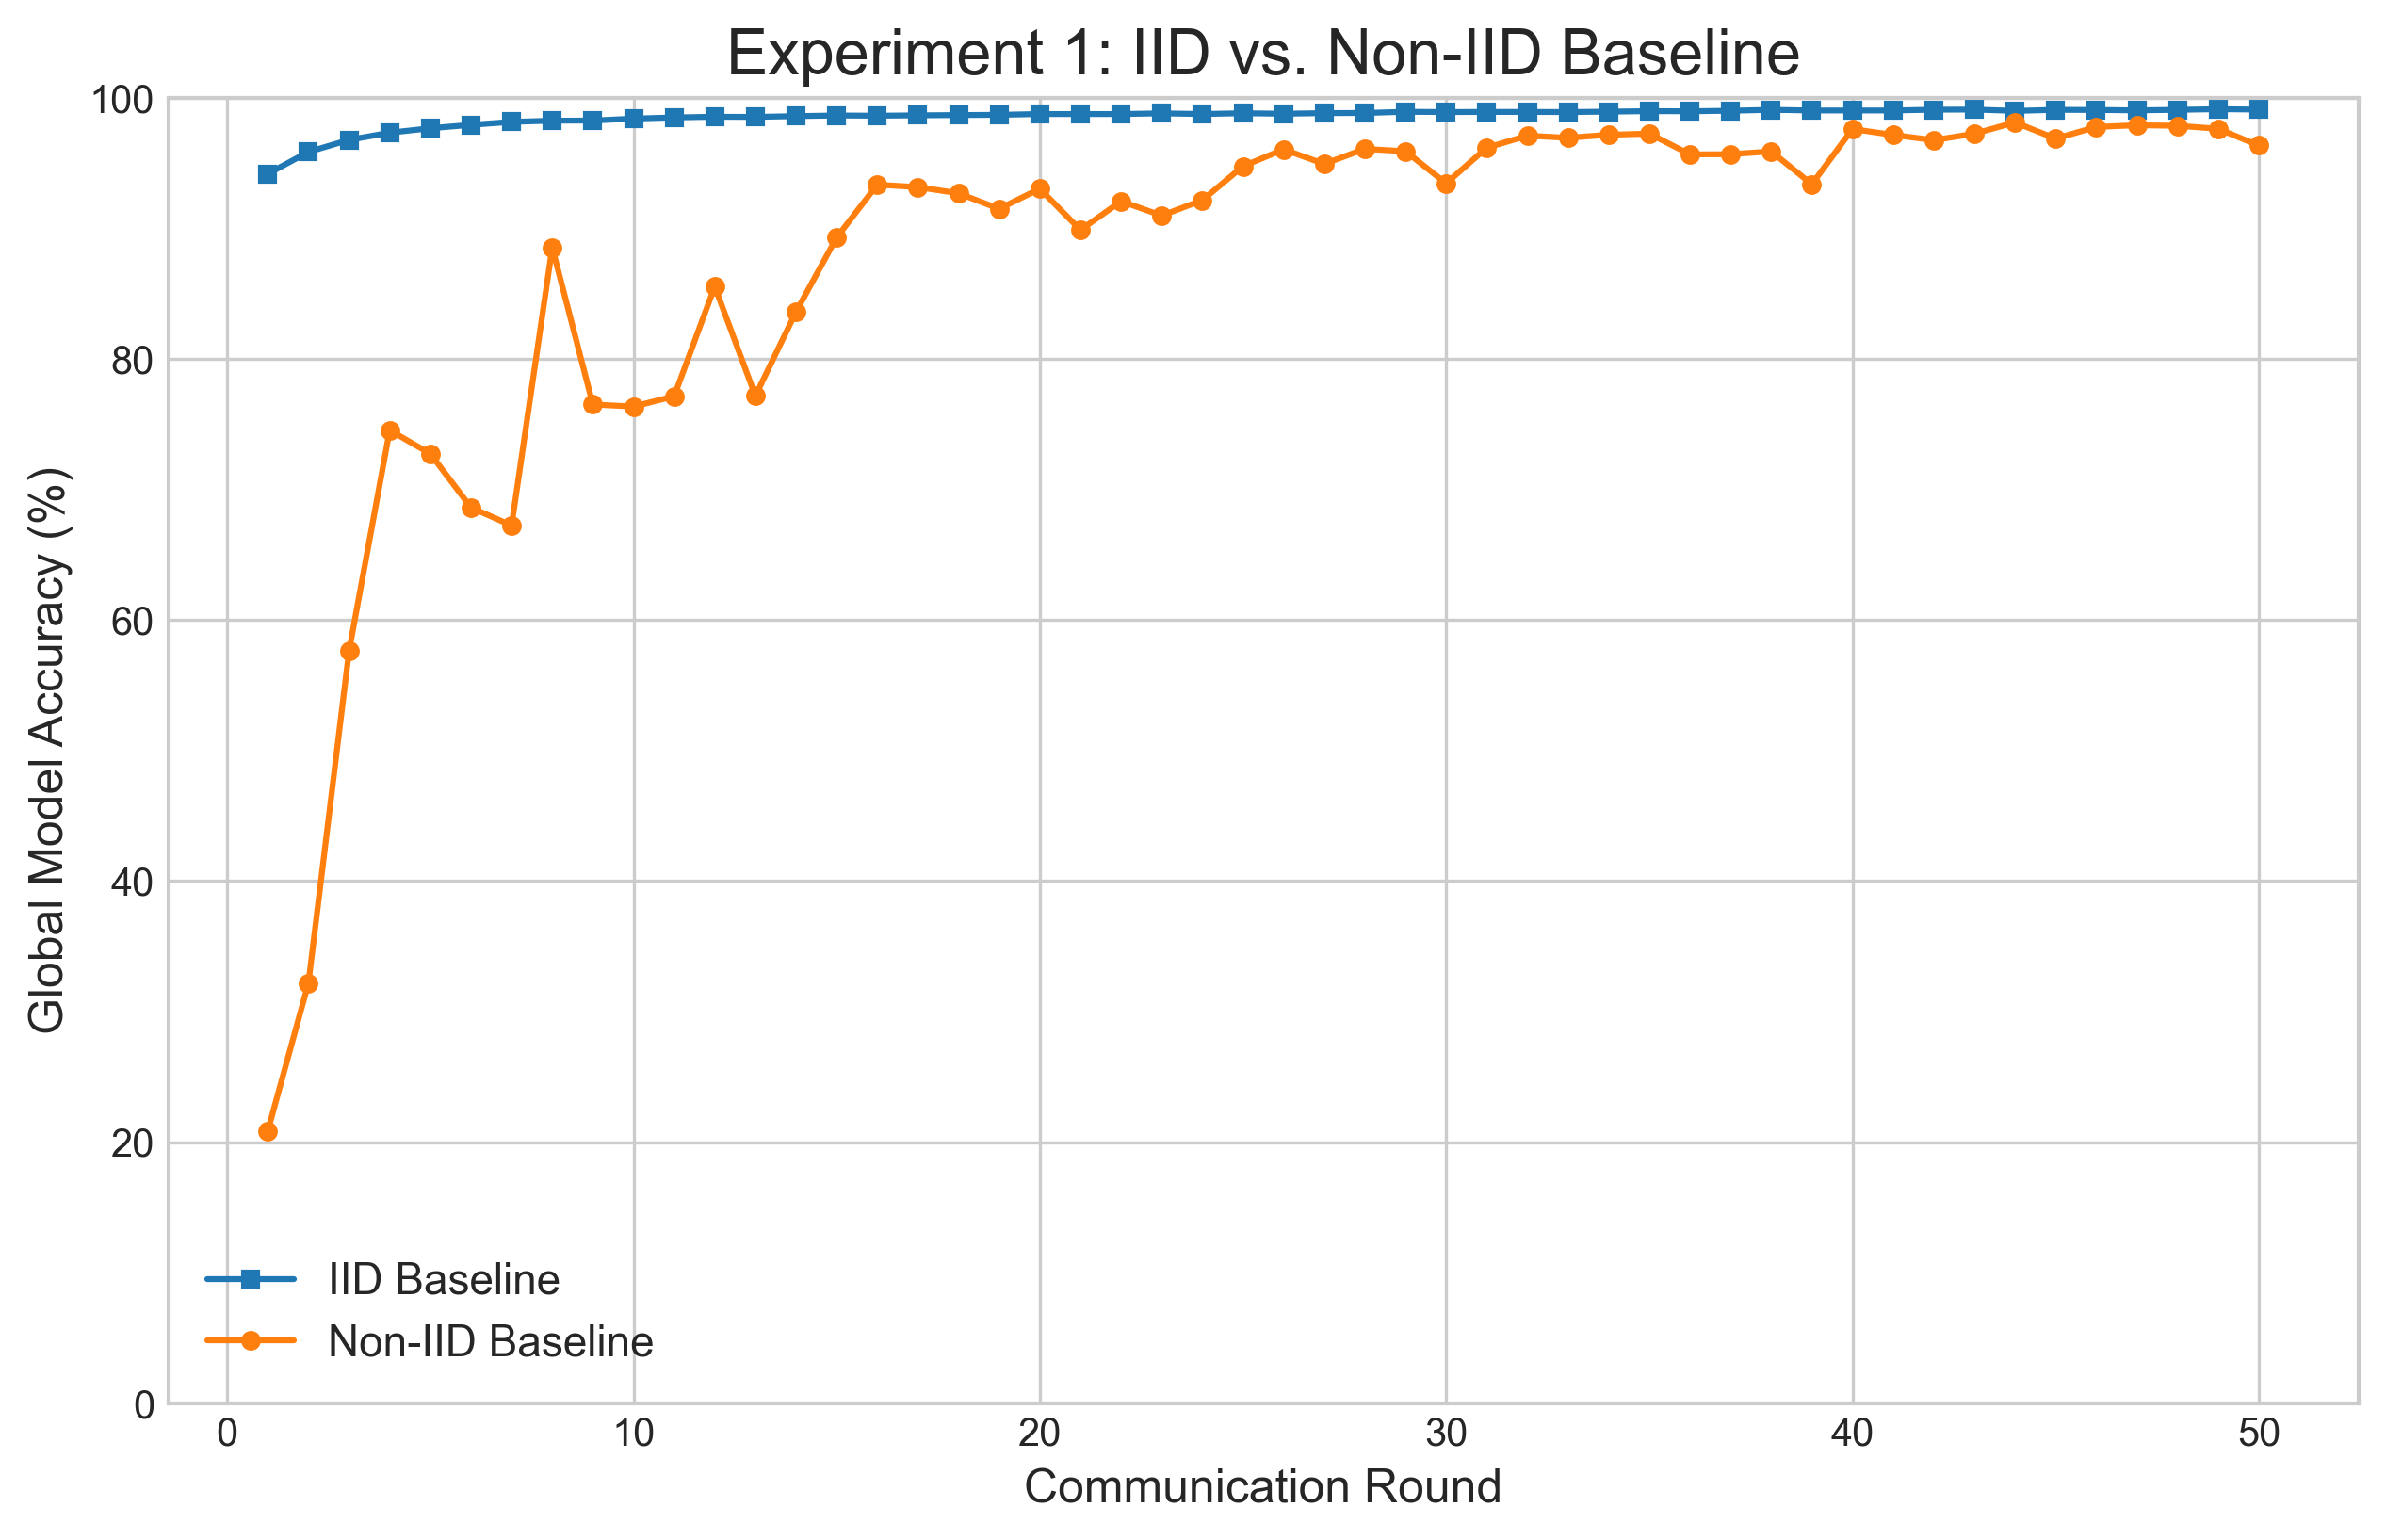
\includegraphics[width=0.9\linewidth]{fig_1_iid_vs_non_iid} % Removed .png extension
  \caption{Experiment 1: Global model accuracy on IID vs. Non-IID data. (C=0.1, E=5 for both).}
  \label{fig:iid}
\end{figure}

% --- FIGURE 2: IMPACT OF C ---
\subsection{Experiment 2: Impact of Client Participation (C)}
Recognizing the instability caused by Non-IID data when averaging updates from only a small fraction of clients ($C=0.1$), we investigated whether increasing this fraction could provide a more stable and representative global update. Figure \ref{fig:impact_c} compares the Non-IID baseline ($C=0.1$, 10 clients per round, blue dashed line, circle markers) with a high participation run ($C=0.5$, 50 clients per round, orange solid line, triangle markers), keeping $E=5$.

The improvement gained by increasing $C$ is substantial. The High-C run ($C=0.5$) exhibits much faster initial learning (reaching over 70\% accuracy by round 3, compared to round 5 for $C=0.1$) and significantly smoother convergence throughout the training process. The large accuracy fluctuations seen in the baseline are almost entirely eliminated. By averaging updates from half the client population each round, the server obtains a much better approximation of the gradient over the *entire* distributed dataset, effectively dampening the conflicting signals from individual clients whose data covers only a small part of the overall distribution. This increased participation acts as a form of variance reduction. Consequently, the final accuracy improves noticeably, rising from 96.34\% to 98.43\% (Table \ref{tab:results}), nearing the performance achieved in the ideal IID case. However, this stability and accuracy come at a significant cost in system resources. As seen in Table \ref{tab:results}, the total simulation time increased dramatically to \SI{8119.42}{s} (over 4 times longer than the baseline). This reflects the fact that five times as many clients performed local computations and (simulated) communication in each round, highlighting the direct trade-off between per-round cost and convergence quality when adjusting $C$.

\begin{figure}[htbp]
  \centering
  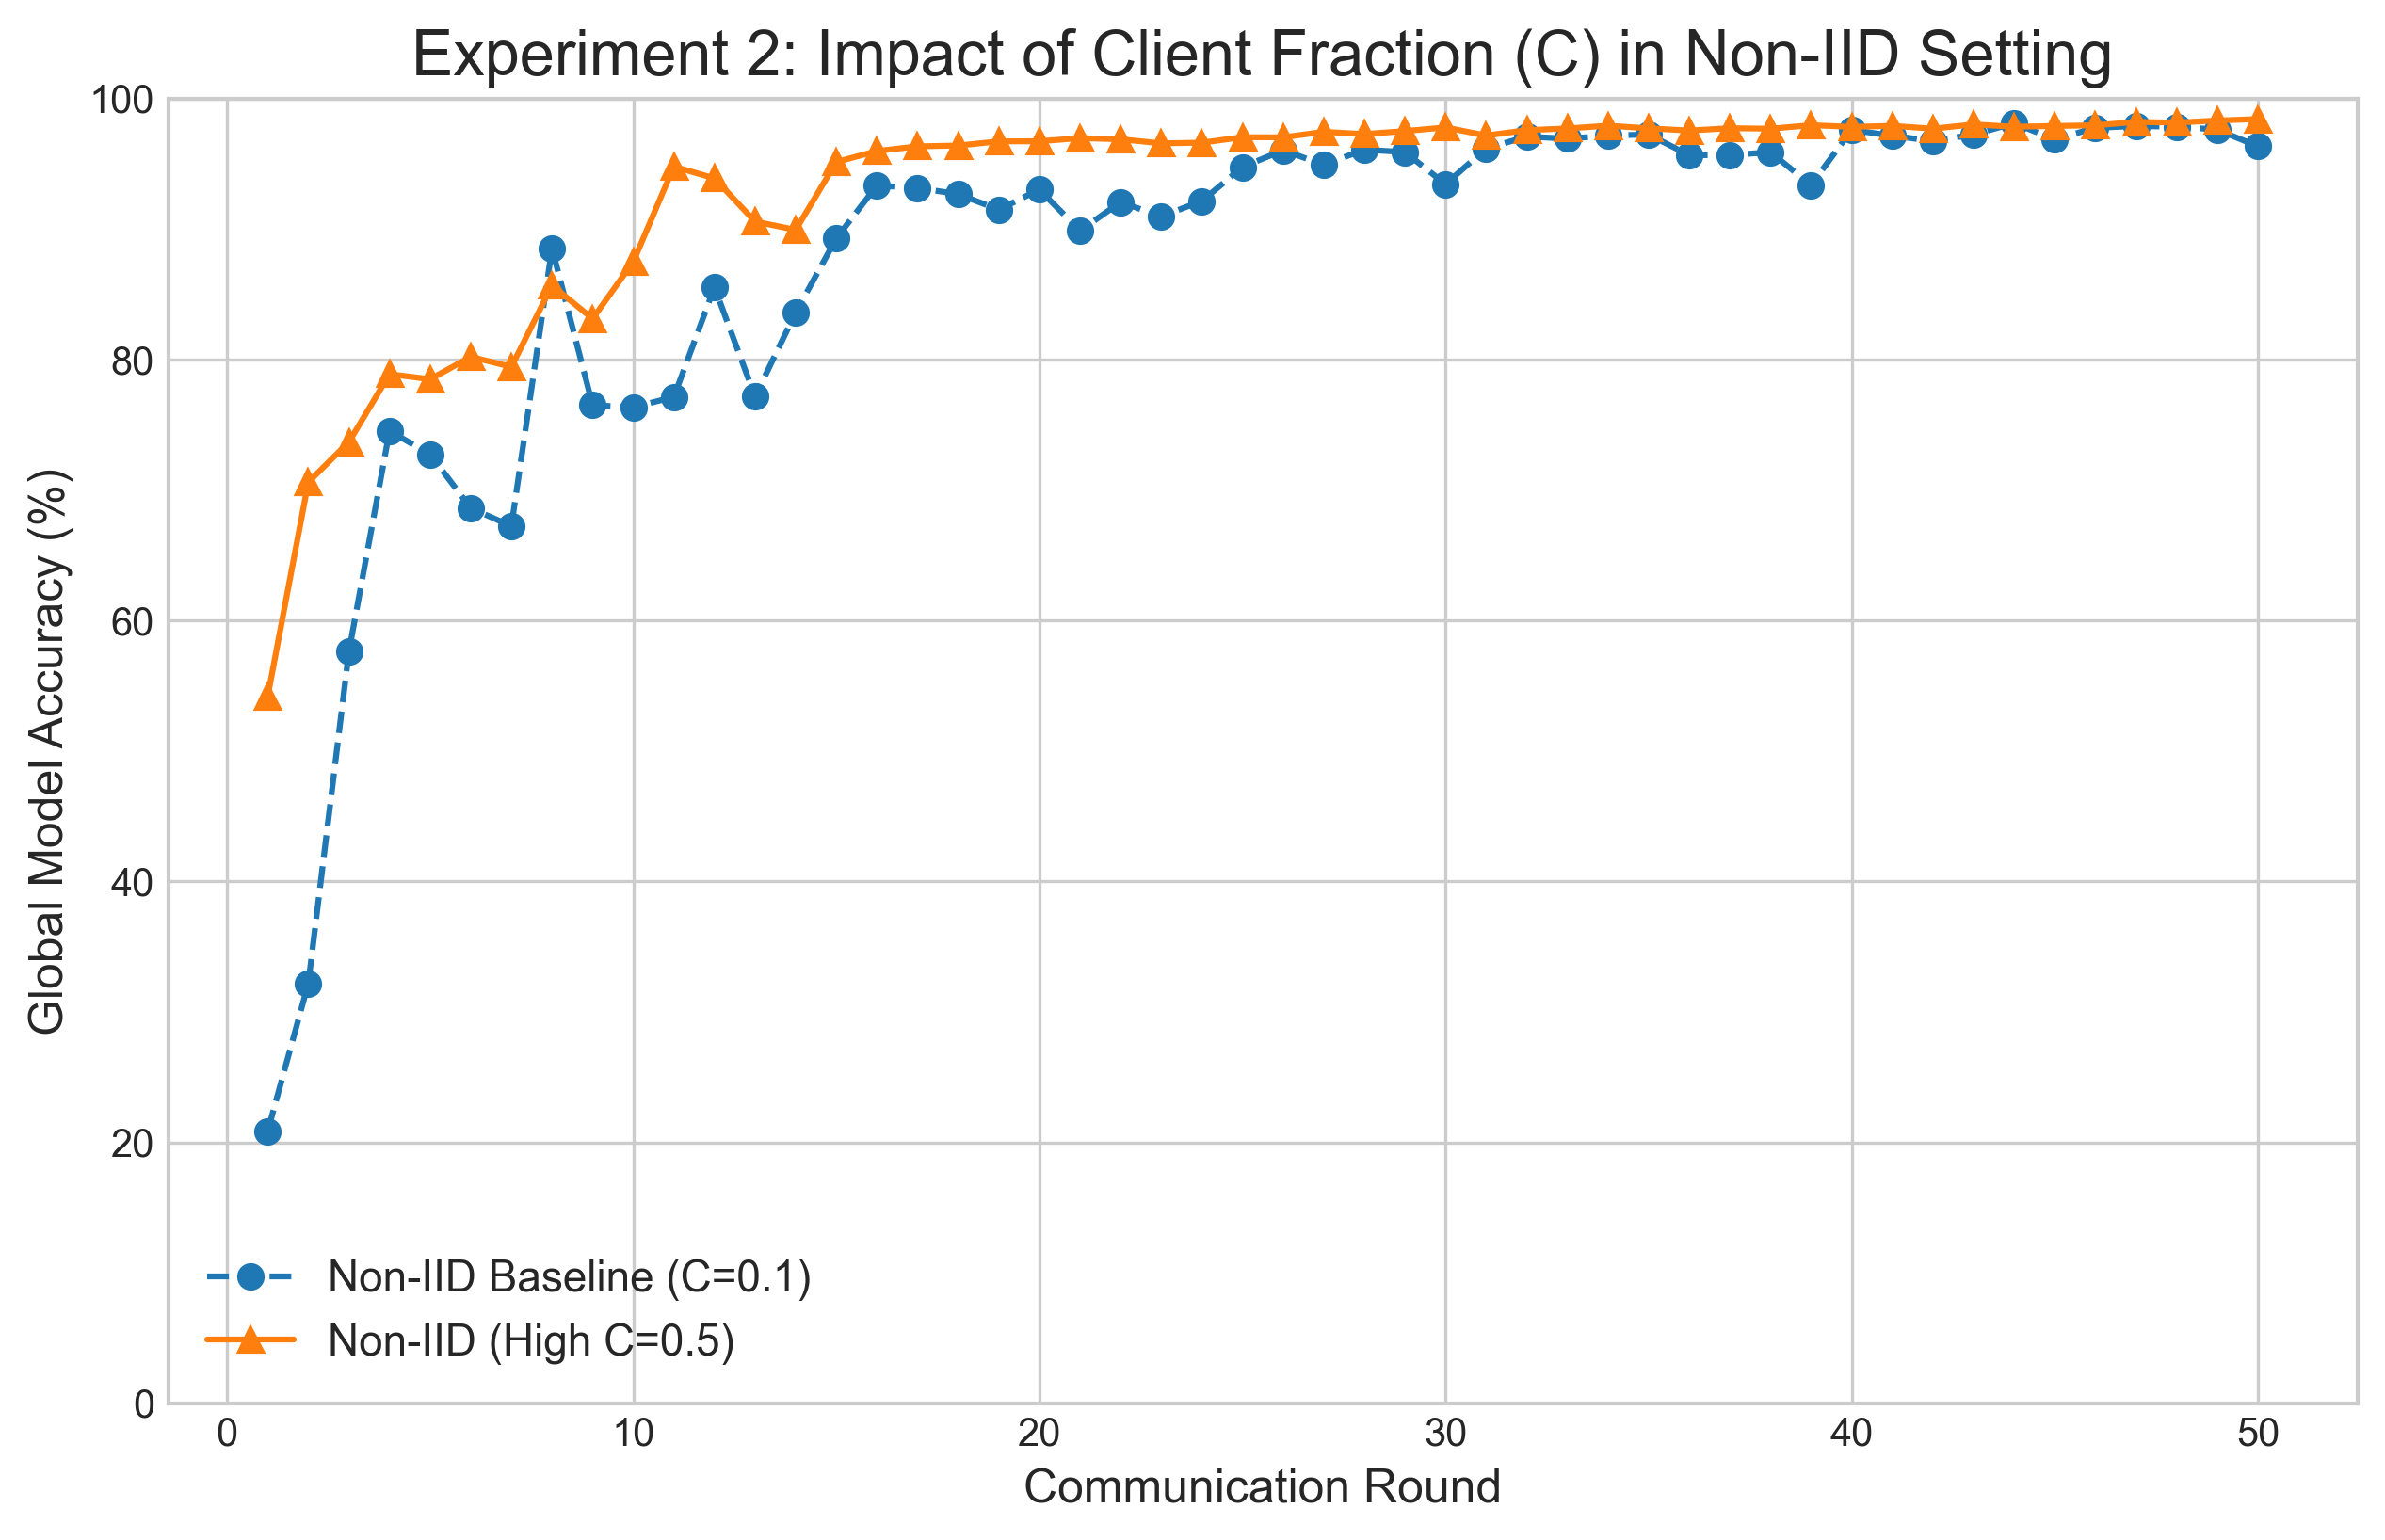
\includegraphics[width=0.9\linewidth]{fig_2_impact_of_C} % Removed .png extension
  \caption{Experiment 2: Impact of client participation (C) in a Non-IID setting. (E=5 for both).}
  \label{fig:impact_c}
\end{figure}

% --- FIGURE 3: IMPACT OF E ---
\subsection{Experiment 3: Impact of Local Epochs (E)}
This experiment explores the critical trade-off between the amount of local computation performed by clients ($E$) and the frequency of communication with the server, shown in Figure \ref{fig:impact_e}. We compare the Non-IID baseline ($E=5$, orange dashed line, circle markers) against runs with fewer local epochs ($E=1$, blue solid line, cross markers) and more local epochs ($E=10$, green dash-dot line, square markers), while keeping the client participation low ($C=0.1$).

Reducing local work to only one epoch ($E=1$, blue line) results in very slow convergence. Clients make minimal progress optimizing their local models before sending updates, meaning many communication rounds are needed for the global model to learn effectively. While the accuracy does increase, it does so much more slowly than the $E=5$ baseline and plateaus at the lowest final accuracy observed in any experiment, only 93.65\%. The only advantage is the significantly reduced simulation time (\SI{475.57}{s}, Table \ref{tab:results}), as clients perform minimal computation. This demonstrates that insufficient local work can severely hinder learning.

Conversely, increasing local work to ten epochs ($E=10$, green line) presents a more complex dynamic. In the initial rounds (up to round 15), this configuration exhibits even greater instability than the $E=5$ baseline, with sharp drops in accuracy (e.g., between rounds 7 and 10). This is a clear manifestation of aggravated client drift: clients train for longer on their highly biased local data, causing their models to diverge further from the (initially poor) global model and from each other. However, after this tumultuous initial phase (around round 20), the model begins to converge rapidly and eventually reaches a high final accuracy (97.74\%), surpassing the $E=5$ baseline. This suggests that while extensive local training exacerbates client drift early on, it might allow clients to find better local optima which, once averaged over enough rounds, contribute to a better final global model. It potentially reduces the *total number of communication rounds* needed to reach a target accuracy compared to lower $E$, but at the cost of higher per-round computation and initial instability. The simulation time (\SI{3223.19}{s}) reflects the doubled local computation compared to $E=5$.

\begin{figure}[htbp]
  \centering
  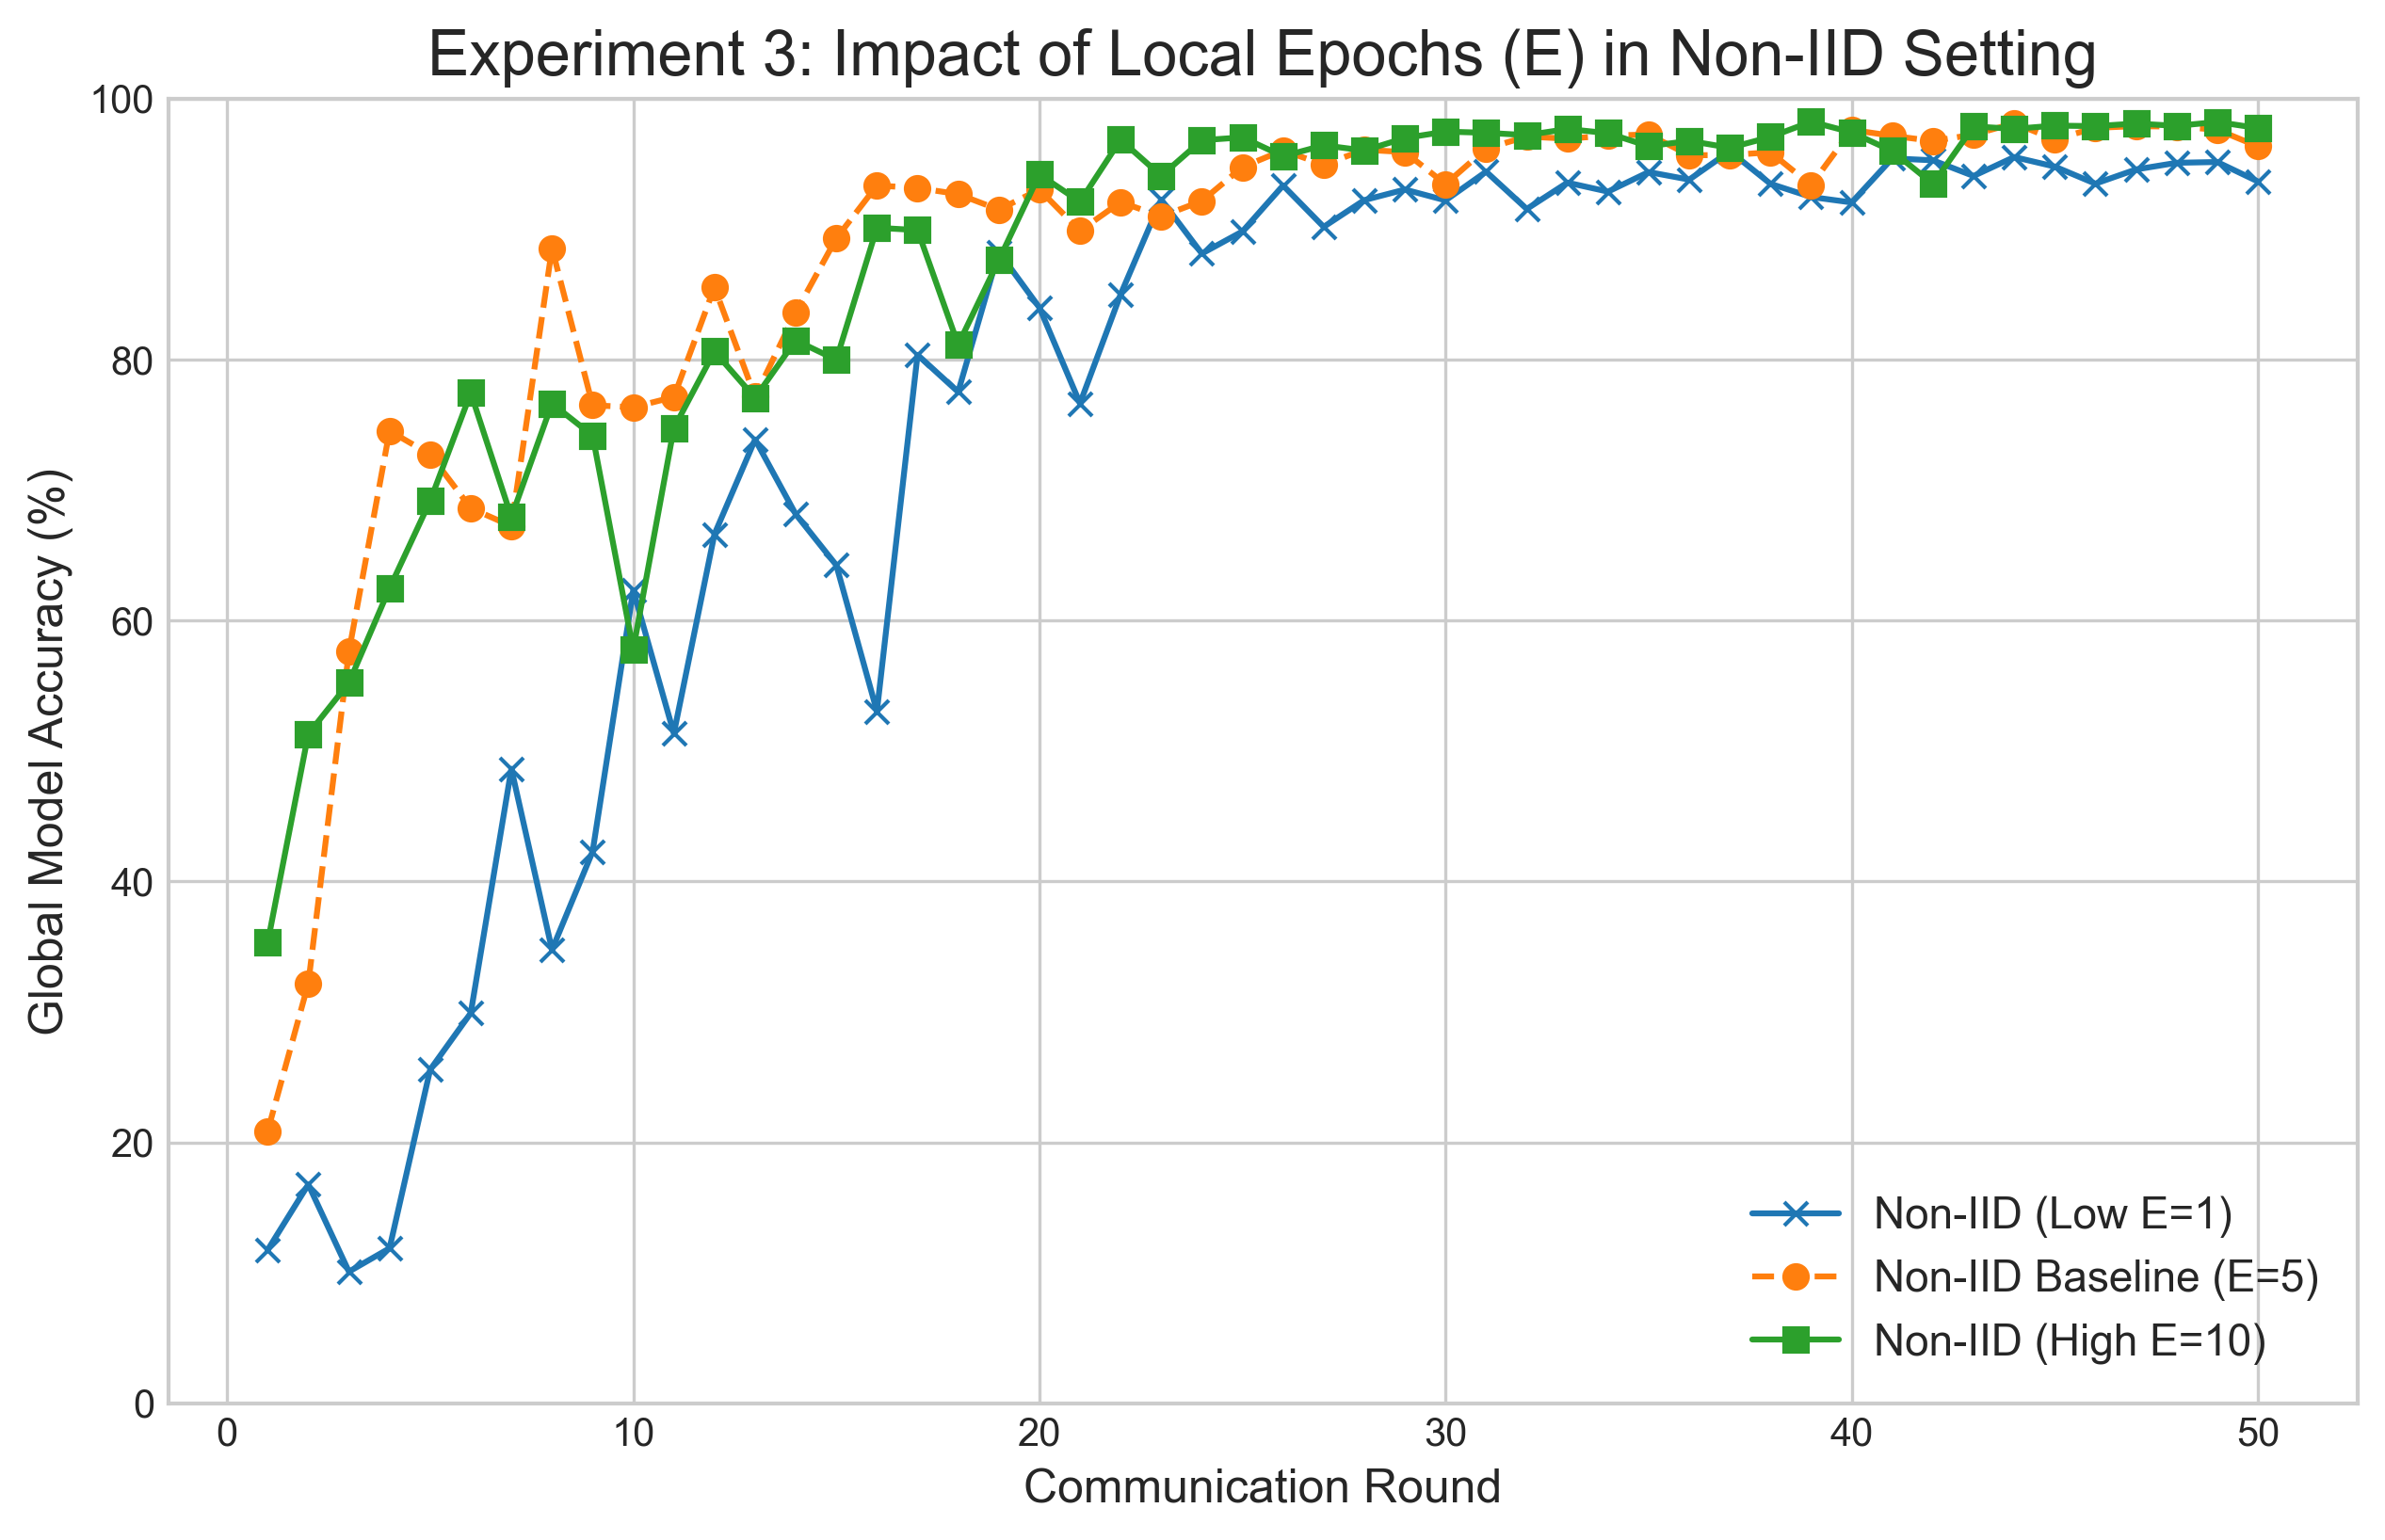
\includegraphics[width=0.9\linewidth]{fig_3_impact_of_E} % Removed .png extension
  \caption{Experiment 3: Impact of local epochs (E) in a Non-IID setting. (C=0.1 for all).}
  \label{fig:impact_e}
\end{figure}

% --- FIGURE 4: COMBINED MITIGATION ---
\subsection{Experiment 4: A Combined Mitigation Strategy}
Drawing insights from the previous experiments—specifically, that high $C$ promotes stability and low $E$ reduces client drift—we hypothesized that combining these two adjustments might yield a robust and efficient configuration for the Non-IID setting. Figure \ref{fig:combined} compares this combined strategy ($C=0.5, E=1$, green dash-dot line, triangle markers) against the IID Baseline (blue dotted line, square markers) and the Non-IID Baseline ($C=0.1, E=5$, orange dashed line, circle markers).

The results strongly support our hypothesis. The combined strategy exhibits remarkably stable convergence, nearly matching the smoothness of the ideal IID baseline after the initial few rounds. It avoids the severe initial instability seen in the Non-IID baseline and the High-E run. Its accuracy quickly surpasses the Non-IID baseline and maintains steady progress throughout the 50 rounds. As shown in Table \ref{tab:results}, the final accuracy (97.42\%) is significantly better than the Non-IID baseline (96.34\%) and approaches the High-E result (97.74%) but without the initial volatility. Crucially, this high performance is achieved with excellent efficiency; the total simulation time (\SI{1720.73}{s}) is comparable to the IID baseline (\SI{1631.88}{s}) and much faster than the High-C, E=5 run (\SI{8119.42}{s}). This approach effectively leverages the variance-reducing benefit of high participation while simultaneously preventing excessive client drift by limiting local computation, suggesting a practical and efficient configuration for tackling Non-IID data with FedAvg.

\begin{figure}[htbp]
  \centering
  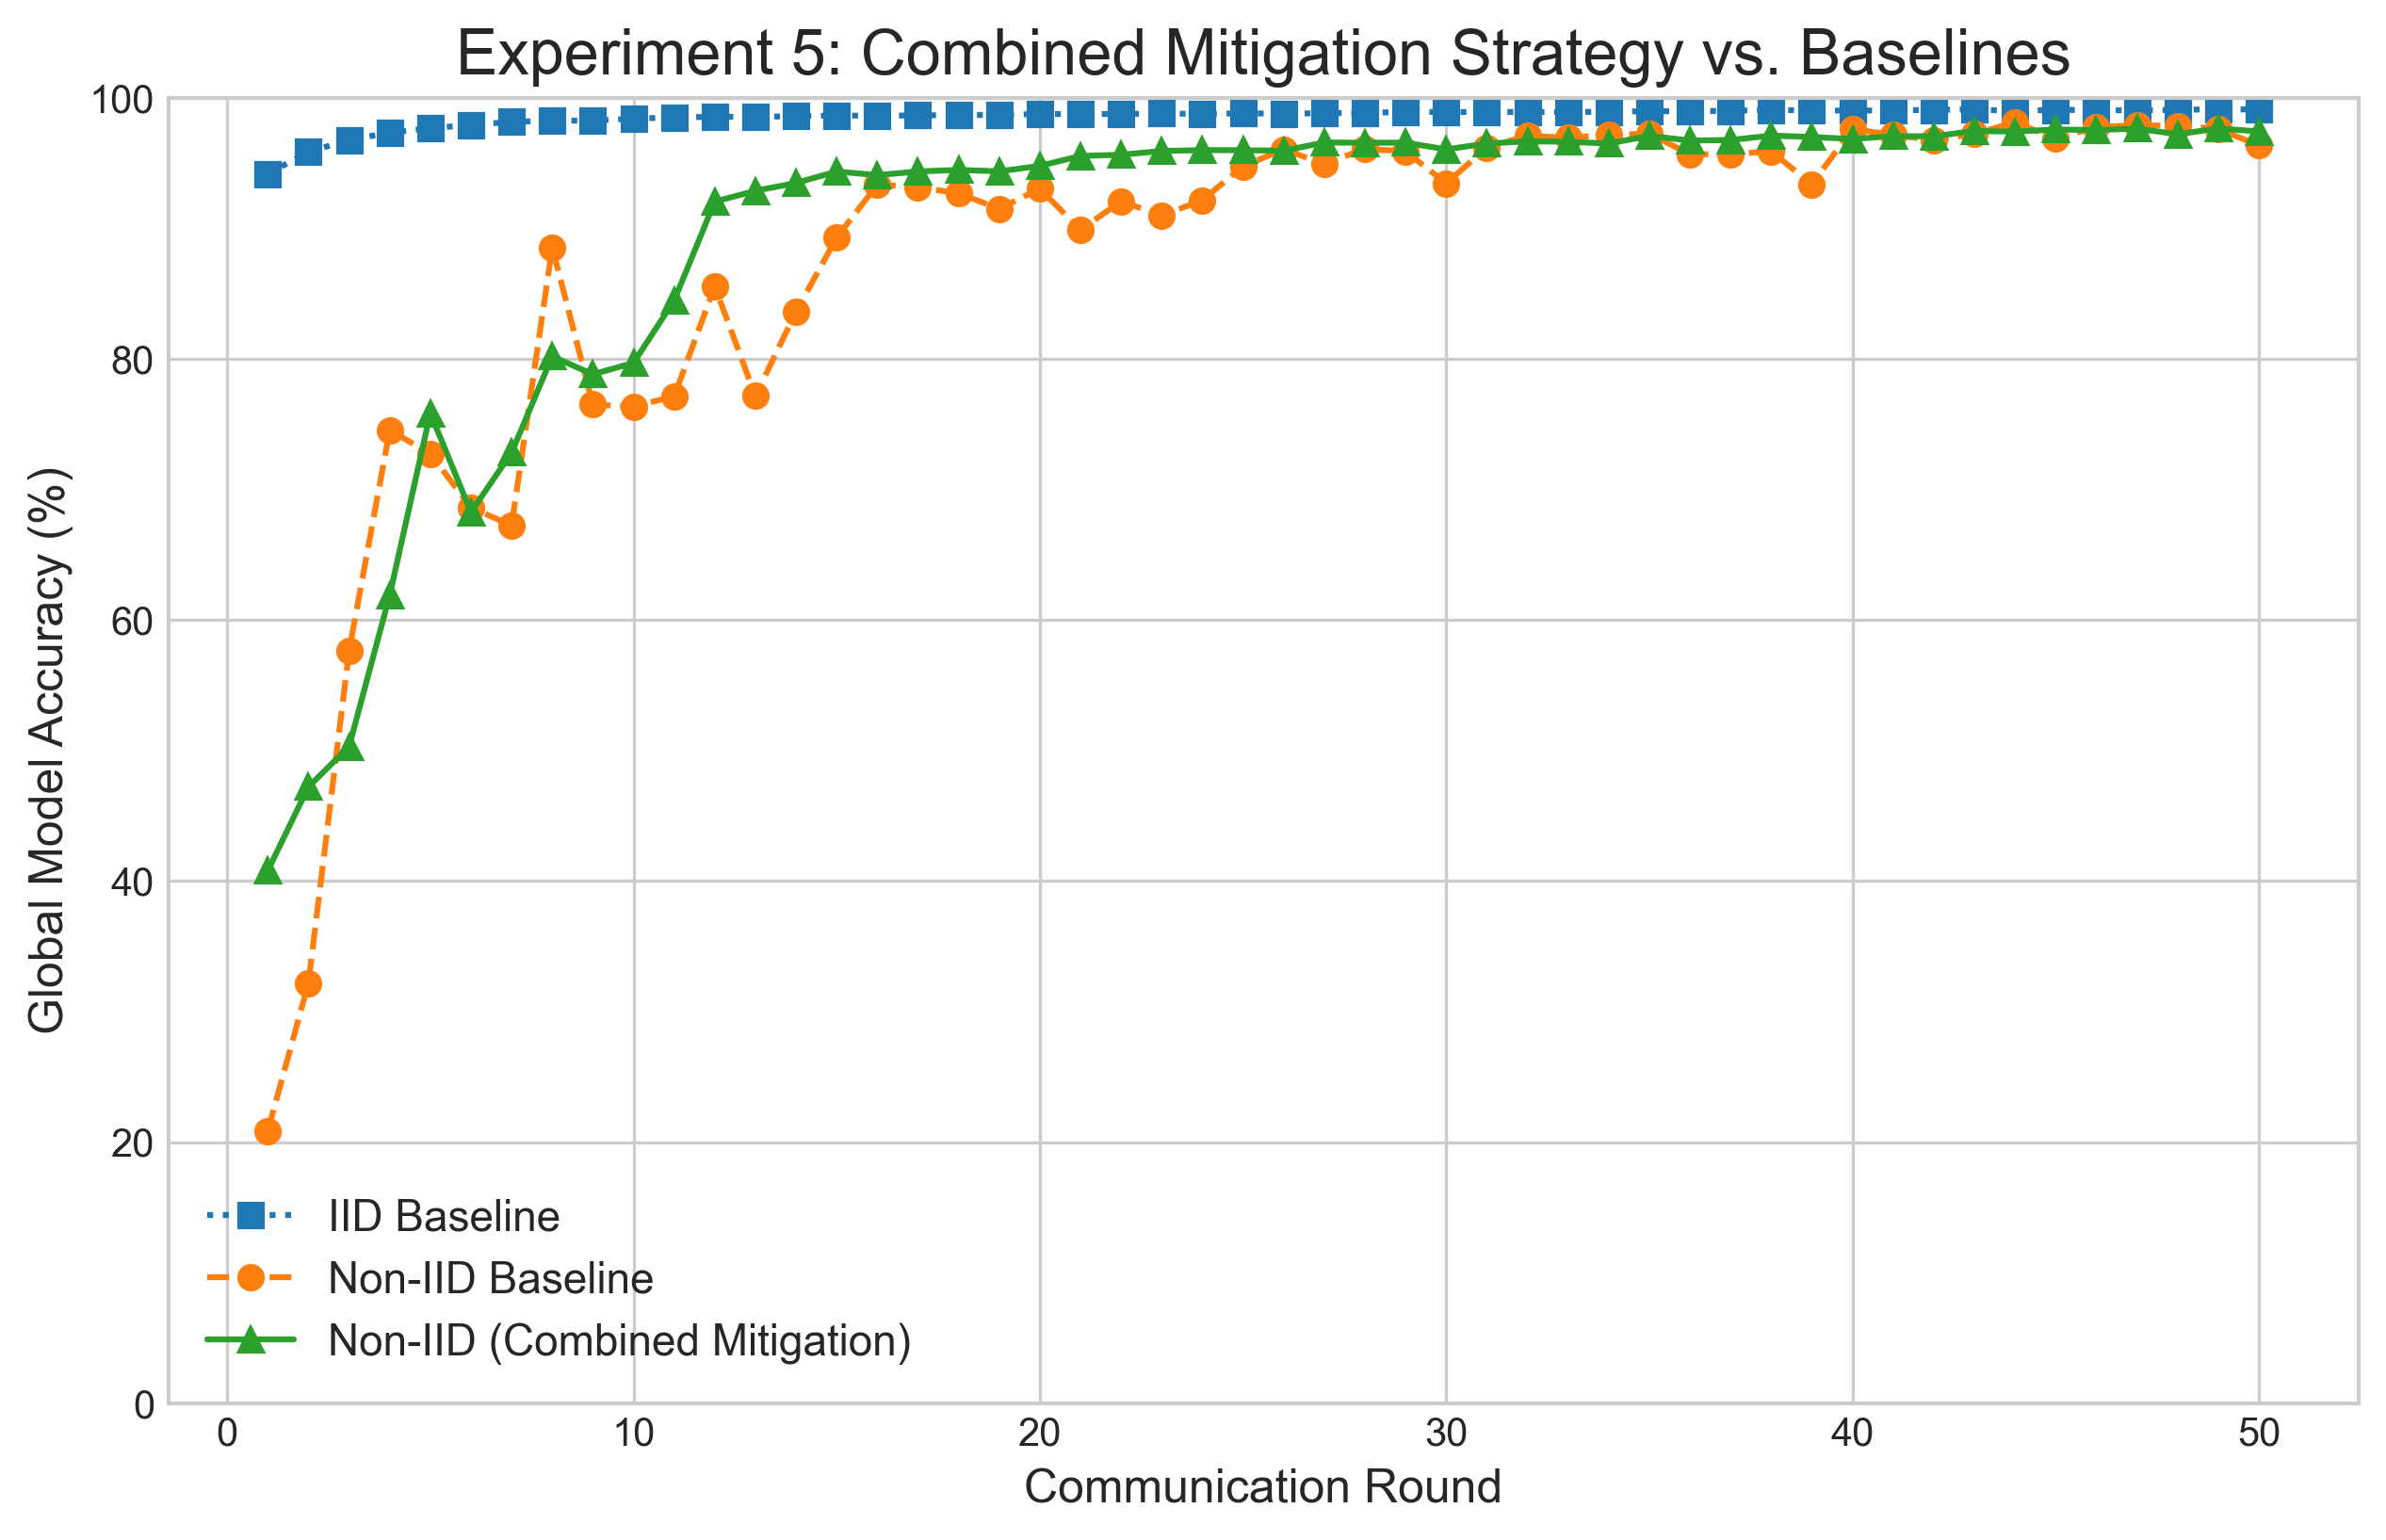
\includegraphics[width=0.9\linewidth]{fig_5_combined_mitigation} % Removed .png extension
  \caption{Experiment 4: Combined mitigation (C=0.5, E=1) vs. the IID and Non-IID baselines.}
  \label{fig:combined}
\end{figure}


% --- DISCUSSION ---
\section{Discussion}
Our simulation results provide valuable insights into how the choice of client participation ($C$) and local epochs ($E$) influences the behavior of clients, the server, and the overall training process in Federated Learning, particularly when dealing with Non-IID data.

\subsection{Impact on Clients}
The parameters $C$ and $E$ directly dictate the experience and workload of the participating clients.
\begin{itemize}
    \item \textbf{Workload per Round:} The number of local epochs ($E$) determines the computational effort required from a client *if selected* in a given round. Higher $E$ means more training iterations, more computation time, and potentially higher energy consumption on the client device. Our simulations reflect this: the High-E ($E=10$) run took roughly twice as long as the baseline ($E=5$), while the Low-E ($E=1$) run was significantly faster (Table \ref{tab:results}).
    \item \textbf{Probability of Participation:} The client participation fraction ($C$) determines how often, on average, a given client is selected to participate. A low $C$ (like 0.1) means a client is only involved occasionally, reducing its overall burden but also meaning its data contributes less frequently to the global model. A high $C$ (like 0.5) means clients participate much more often, increasing their overall contribution but also their total workload.
    \item \textbf{Client Drift:} For clients with Non-IID data, a high $E$ increases the risk of their local model significantly diverging ("drifting") from the global objective. As seen in Figure \ref{fig:impact_e}, the $E=10$ run showed greater initial instability, likely because individual clients were overfitting to their limited digit classes before their updates were averaged. Conversely, low $E$ ($E=1$) limits this drift but may prevent clients from making meaningful progress.
    \item \textbf{Communication Frequency:} $E$ inversely affects communication frequency. A higher $E$ means clients perform more computation between communication rounds, reducing the total number of rounds potentially needed but increasing the computation per round. A lower $E$ means more frequent communication.
\end{itemize}
Essentially, $E$ controls the computation-communication trade-off *for participating clients*, while $C$ controls how many clients face this trade-off in each round.

\subsection{Impact on the Server}
The server's role is primarily coordination and aggregation, and it is also significantly affected by $C$ and $E$.
\begin{itemize}
    \item \textbf{Aggregation Load:} The client participation fraction ($C$) directly impacts the server's workload per round. Higher $C$ means the server must receive, process, and aggregate updates from more clients. In our $C=0.5$ experiments, the server averaged 50 updates per round, compared to only 10 in the $C=0.1$ runs. This increases the server's computational burden for aggregation and potentially the network bandwidth required to receive updates simultaneously (in a real system).
    \item \textbf{Quality of Aggregated Update:} A higher $C$ generally provides the server with a higher-quality, more stable global update, especially with Non-IID data. Averaging over a larger, more diverse set of clients reduces the variance and bias introduced by any single client's skewed data (as seen in Figure \ref{fig:impact_c}). The number of local epochs ($E$) influences the *content* of the updates the server receives. High $E$ in Non-IID settings can lead to the server receiving highly diverged updates, making the simple averaging process less effective and potentially causing instability (Figure \ref{fig:impact_e}, early rounds of $E=10$).
    \item \textbf{Coordination and Scalability:} While not explicitly modeled in our simulation time, managing communication with a larger number of clients per round (high $C$) poses greater system challenges in a real-world deployment regarding network orchestration, handling stragglers, and potential timeouts.
\end{itemize}
The server benefits from the stability provided by high $C$, but at the cost of increased per-round processing. It also benefits from the faster potential convergence (in terms of rounds) from higher $E$, but risks receiving less coherent updates that hinder aggregation.

\subsection{Impact on Overall Training Process}
The interplay between client actions (driven by $E$) and server aggregation (influenced by $C$ and the quality of updates received) determines the overall training dynamics.
\begin{itemize}
    \item \textbf{Convergence Speed (Rounds):} Non-IID data drastically slows convergence compared to IID (Figure \ref{fig:iid}). High $C$ significantly accelerates convergence in the Non-IID setting (Figure \ref{fig:impact_c}). Low $E$ ($E=1$) results in very slow convergence, while High $E$ ($E=10$), despite initial instability, can sometimes converge in fewer rounds than moderate $E$ ($E=5$) after stabilizing (Figure \ref{fig:impact_e}).
    \item \textbf{Convergence Stability:} IID data leads to smooth convergence. Non-IID data introduces instability, especially with low $C$ and high $E$ (Figure \ref{fig:iid}, \ref{fig:impact_e}). Increasing $C$ is the most effective way to improve stability (Figure \ref{fig:impact_c}). The combination $C=0.5, E=1$ yielded stability almost matching the IID case (Figure \ref{fig:combined}).
    \item \textbf{Final Accuracy:} Non-IID data reduces the achievable accuracy compared to IID. Increasing $C$ generally improves final accuracy in the Non-IID setting (Table \ref{tab:results}). The effect of $E$ is non-monotonic: $E=1$ gave the worst accuracy, while $E=10$ slightly outperformed $E=5$ in our specific runs, but the optimal $E$ likely depends on other factors like the dataset and learning rate.
    \item \textbf{Overall Efficiency (Time):} Total time depends on both the number of rounds and the work per round. High $C$ greatly increases time due to more client computations per round. High $E$ increases time due to more local work per client. Low $E$ is fastest but yields poor results. The combined strategy ($C=0.5, E=1$) provided a good balance, achieving high accuracy and stability in a time comparable to the IID baseline, suggesting it's an efficient configuration for this specific problem.
\end{itemize}
Ultimately, tuning $C$ and $E$ requires balancing the desire for fast convergence (fewer rounds, potentially higher $E$), stability (higher $C$, lower $E$), high final accuracy (often higher $C$), and system resource constraints (communication bandwidth limits $C$, client computation limits $E$). Our results highlight that addressing the Non-IID challenge often involves increasing participation ($C$) while carefully managing local computation ($E$) to prevent client drift.

\subsection{Limitations of this Study}
As a student project based on simulation, this study has several limitations that should be acknowledged:
\begin{itemize}
    \item \textbf{Dataset and Model Simplicity:} MNIST is a relatively easy dataset, and our CNN is small. The observed parameter sensitivities might differ significantly on more complex tasks (e.g., natural language processing) or with larger models (e.g., Transformers, ResNets).
    \item \textbf{Simplified Non-IID:} We used a common but specific method (class partitioning) to create Non-IID data. Real-world heterogeneity can be much more complex, involving feature distribution skew, varying data quantities, and concept drift over time.
    \item \textbf{Idealized Simulation:} Our simulation assumes perfect client availability, reliable communication, and uniform client hardware. Real FL deployments face challenges like client dropouts ("stragglers"), network latency variation, and heterogeneous compute capabilities, which we did not model. Simulation time primarily reflected CPU load, not realistic communication delays.
    \item \textbf{Basic Algorithm:} We only studied the standard FedAvg algorithm. More advanced FL algorithms (e.g., FedProx \cite{b8}, Scaffold \cite{b7}) are specifically designed to better handle Non-IID data and might show different sensitivities to $C$ and $E$.
    \item \textbf{Limited Hyperparameters:} We only varied $C$ and $E$, keeping factors like learning rate and batch size fixed. A full exploration would involve tuning these as well.
\end{itemize}
Despite these limitations, the study provides a valuable illustration of core FL principles and parameter effects in a controlled environment.


% --- CONCLUSION ---
\section{Conclusion and Future Work}
This paper presented an empirical investigation into the effects of fundamental parameters within the Federated Averaging (FedAvg) algorithm, specifically focusing on the client participation rate ($C$) and the number of local training epochs ($E$). Motivated by the increasing importance of privacy-preserving machine learning and the inherent challenges of decentralized data, particularly Non-IID distributions, we utilized a simulation environment with the MNIST dataset and a standard CNN model to systematically analyze these parameters' impact on model performance and training dynamics. Our work aimed to reproduce and clearly illustrate known FL behaviors for educational and baseline purposes.

Our simulations successfully demonstrated the critical role these parameters play in the FedAvg framework. We quantitatively confirmed the significant performance penalty imposed by Non-IID data, observing a marked decrease in final accuracy (from 99.09\% down to 96.34\% in our baseline tests) and pronounced instability during convergence compared to the ideal IID scenario, as clearly visualized in Figure \ref{fig:iid}. This underscores the necessity of considering data heterogeneity when designing and tuning FL systems.

Investigating mitigation strategies, we found that increasing client participation ($C=0.5$ vs $C=0.1$) substantially improved performance, boosting accuracy to 98.43\% and significantly smoothing the learning curve (Figure \ref{fig:impact_c}). This supports the intuition that averaging updates from a larger, more diverse set of clients helps counteract individual biases and leads to a more stable global update. However, this benefit came at the cost of a considerable increase in per-round computational load and overall simulation time (Table \ref{tab:results}).

Conversely, our study of local epochs ($E$) highlighted a complex trade-off. Minimal local work ($E=1$) resulted in very slow learning and the lowest final accuracy (93.65\%), indicating insufficient local model refinement between communication rounds. Extensive local work ($E=10$), while achieving a high final accuracy (97.74\%), exacerbated client drift, leading to significant instability, especially in the early stages of training (Figure \ref{fig:impact_e}). This suggests a delicate balance is required: enough local training is needed for progress, but too much can cause local models to diverge detrimentally on biased data.

Importantly, our "Combined Mitigation" experiment ($C=0.5, E=1$) demonstrated a highly effective strategy within our simulation context. It achieved robust stability, high accuracy (97.42\%), and efficient convergence comparable in time to the IID baseline (Figure \ref{fig:combined}, Table \ref{tab:results}). This finding suggests that frequent aggregation ($E=1$) of updates from a large client pool ($C=0.5$) can be a practical approach to harnessing the benefits of broad participation while actively suppressing client drift, offering a valuable configuration pattern for dealing with Non-IID data using FedAvg.

In summary, this project provides tangible, empirical evidence illustrating the fundamental trade-offs associated with key FedAvg parameters. It emphasizes that optimizing FL is not straightforward and requires balancing accuracy, stability, communication overhead, and computational cost, particularly in the face of statistical heterogeneity. While framed within the limitations of our specific simulation setup (MNIST, simple CNN, idealized conditions), the observed dynamics offer valuable practical insights and a foundational understanding for further exploration into Federated Learning.

Future work could meaningfully extend this investigation. Repeating these experiments on more challenging datasets (e.g., CIFAR-10 with its color images and more complex classes, or text datasets like Sentiment140) and using more sophisticated model architectures (e.g., ResNet variants) would be essential to assess the generalizability of our findings regarding $C$ and $E$. Implementing and rigorously comparing the performance of advanced FL algorithms specifically designed to combat heterogeneity (such as FedProx \cite{b8}, Scaffold \cite{b7}, or FedNova \cite{b19}) against our FedAvg baseline under identical Non-IID conditions would quantify their practical advantages. Furthermore, enhancing the simulation to model system-level complexities, such as client dropouts (stragglers), variable network bandwidth, or differing client computational capabilities, would significantly increase the fidelity and real-world relevance of the study.


% --- REFERENCES ---
% (References remain the same as previous version)
\begin{thebibliography}{1}
\providecommand{\url}[1]{#1}
\csname url@samestyle\endcsname
\providecommand{\newblock}{\relax}
\providecommand{\bibinfo}[2]{#2}
\providecommand{\BIBentrySTDinterwordspacing}{\spaceskip=0pt\relax}
\providecommand{\BIBentryALTinterwordstretchfactor}{4}
\providecommand{\BIBentryALTinterwordspacing}{\spaceskip=\fontdimen2\font plus
\BIBentryALTinterwordstretchfactor\fontdimen3\font minus
  \fontdimen4\font\relax}
\providecommand{\BIBforeignlanguage}[2]{{%
\expandafter\ifx\csname l@#1\endcsname\relax
\typeout{** WARNING: IEEEtran.bst: No hyphenation pattern has been}%
\typeout{** loaded for the language `#1'. Using the default patterns.}%
\fi
\language=\csname l@#1\endcsname
\boldgroup
\emph{#2}%
\egroup
}}
\providecommand{\BIBdecl}{\relax}
\BIBdecl

\bibitem{b1}
R.~Shokri and V.~Shmatikov, ``Privacy-preserving deep learning,'' in
  \emph{Proceedings of the 22nd ACM SIGSAC Conference on Computer and
  Communications Security}, 2015, pp. 1310--1321.

\bibitem{b2}
H.~B. McMahan, E.~Moore, D.~Ramage, S.~Hampson, and B.~A. y~Arcas,
  ``Communication-efficient learning of deep networks from decentralized data,''
  in \emph{Proceedings of the 20th International Conference on Artificial
  Intelligence and Statistics (AISTATS)}, 2017.

\bibitem{b3}
V.~J. K. K. S. M.~Z. J.~Konečný, H.~B. McMahan, ``Federated learning: Strategies
  for improving communication efficiency,'' \emph{arXiv preprint
  arXiv:1610.05492}, 2016.

\bibitem{b4}
Y.~LeCun, L.~Bottou, Y.~Bengio, and P.~Haffner, ``Gradient-based learning
  applied to document recognition,'' \emph{Proceedings of the IEEE}, vol.~86,
  no.~11, pp. 2278--2324, 1998.

\bibitem{b5}
J.~Konečný, H.~B. McMahan, F.~X. Yu, P.~Richtárik, A.~T. Suresh, and D.~Bacon,
  ``Federated learning: Strategies for improving communication efficiency,''
  \emph{arXiv preprint arXiv:1610.05492}, 2016.

\bibitem{b6}
P.~Reisizadeh, A.~Mokhtari, H.~Hassani, A.~Sarwate, and R.~K. P.
  ``Fedpaq: A communication-efficient federated learning method,'' \emph{arXiv
  preprint arXiv:1905.06053}, 2019.

\bibitem{b7}
S.~P. Karimireddy, S.~Konečný, K.~M. J.~Reddi, S.~J., and A.~Stich, ``Scaffold:
  Stochastic controlled averaging for federated learning,'' in \emph{Proceedings
  of the 37th International Conference on Machine Learning (ICML)}, 2020.

\bibitem{b8}
T.~Li, A.~K. Sahu, A.~Talwalkar, and V.~Smith, ``Fedprox: Federated
  optimization with convex constraints,'' \emph{arXiv preprint
  arXiv:1812.06127}, 2018.

\bibitem{b9}
S.~J. Reddi, J.~Konečný, K.~M. S.~P., and A.~Stich, ``Adaptive federated
  optimization,'' \emph{arXiv preprint arXiv:2003.00295}, 2020.

\bibitem{b10}
Z.~Charles, Z.~Garrett, R.~M. K.~S., and H.~B. McMahan, ``On the convergence of
  federated averaging on non-iid data,'' \emph{arXiv preprint
  arXiv:1907.02189}, 2019.

\bibitem{b11}
E.~Bagdasaryan, A.~Veit, Y.~Hua, D.~Stutz, and V.~Shmatikov, ``How to backdoor
  federated learning,'' in \emph{Proceedings of the 23rd International
  Conference on Artificial Intelligence and Statistics (AISTATS)}, 2020.

\bibitem{b12}
L.~Zhu, Z.~Liu, and S.~Han, ``Deep leakage from gradients,'' in
  \emph{Proceedings of the 33rd Conference on Neural Information Processing
  Systems (NeurIPS)}, 2019.

\bibitem{b13}
K.~Bonawitz, V.~Ivanov, B.~Kreuter, A.~Marcedone, H.~B. McMahan, S.~Patel,
  D.~Ramage, A.~Segal, and K.~Seth, ``Practical secure aggregation for
  privacy-preserving machine learning,'' in \emph{Proceedings of the 2017 ACM
  SIGSAC Conference on Computer and Communications Security (CCS)}, 2017.

\bibitem{b14}
R.~C. Geyer, T.~Kopelowitz, and D.~Stanton, ``Differentially private federated
  learning: A client level perspective,'' \emph{arXiv preprint
  arXiv:1712.07557}, 2017.

\bibitem{b15}
H.~B. McMahan, D.~Ramage, K.~Talwar, and L.~Zhang, ``Learning
  differentially private recurrent language models,'' \emph{arXiv preprint
  arXiv:1710.06963}, 2017.

\bibitem{b16}
F.~Sattler, K.-R. Müller, and W.~Samek, ``Clustered federated learning:
  Model-agnostic distributed multitask learning under data heterogeneity,''
  \emph{IEEE Transactions on Neural Networks and Learning Systems}, 2020.

\bibitem{b17}
A.~Paszke \emph{et~al.}, ``Pytorch: An imperative style, high-performance deep
  learning library,'' in \emph{Advances in Neural Information Processing Systems
  32 (NeurIPS)}, 2019, pp. 8024--8035.

\bibitem{b18}
X.~Li, K.~Huang, W.~Yang, S.~Wang, and Z.~Zhang, ``On the convergence of
  fedavg on non-iid data,'' \emph{arXiv preprint arXiv:1907.02189}, 2019.

\bibitem{b19}
S.~Wang, T.~Tu, A.~T. S.~H., and V.~Smith, ``Adaptive federated learning in
  resource constrained edge computing systems,'' \emph{IEEE Journal on Selected
  Areas in Communications}, vol.~37, no.~6, pp. 1205--1221, 2019.

\bibitem{b20}
F.~Sattler, S.~Wiedemann, K.-R. Müller, and W.~Samek, ``Robust and
  communication-efficient federated learning from non-iid data,'' \emph{IEEE
  Transactions on Neural Networks and Learning Systems}, vol.~31, no.~9, pp.
  3400--3413, 2019.

\bibitem{b21}
J.~Konečný and H.~B. McMahan, ``Federated learning,'' \emph{Communications of
  the ACM}, vol.~64, no.~4, pp. 58--58, 2021.

\bibitem{b22}
Q.~Yang, Y.~Liu, T.~Chen, and Y.~Tong, ``Federated machine learning: Concept
  and applications,'' \emph{ACM Transactions on Intelligent Systems and
  Technology (TIST)}, vol.~10, no.~2, pp. 1--19, 2019.

\end{thebibliography}




% that's all folks
\end{document}